\section{Basic Functionalities guide}
\subsection{Functional Elements}
\subsubsection{ExternalAPI}
ExternalAPI is a useful element capable to get a JSON file from a API method and to store it in the BubbleMemory. 
\begin{figure}[H]
	\centering
	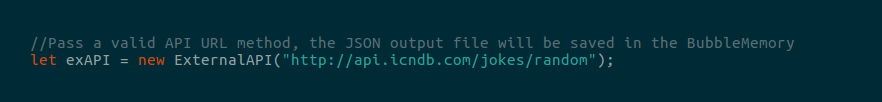
\includegraphics[width=14cm]{../../documenti/UserManualFramework/framework_model/1framework_model_api.png}
	\caption{ExternalAPI}
\end{figure}

\subsubsection{Notification}
Through Notification is possible to show the user a notification, the user can specify a title, an icon and some text to create the notification. 
\begin{figure}[H]
	\centering
	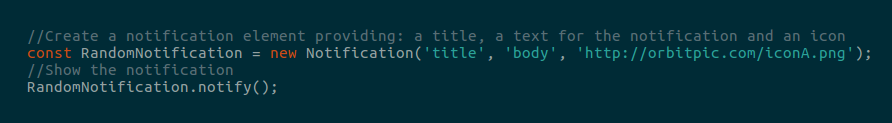
\includegraphics[width=14cm]{../../documenti/UserManualFramework/framework_model/2framework_model_notification.png}
	\caption{Notification}
\end{figure}

\subsubsection{Database}
The functional element Database is based on MongoDB collection system, it is used to write and read data in the collections by simply specifing an url pointing to a MongoDB instance and the name of a collection.
\begin{figure}[H]
	\centering
	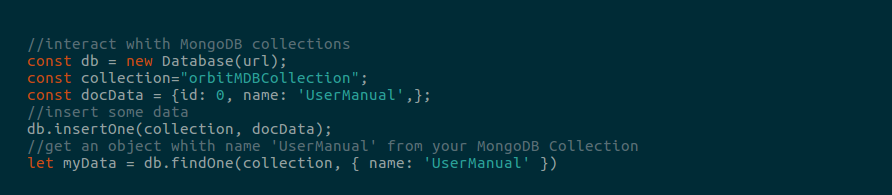
\includegraphics[width=14cm]{../../documenti/UserManualFramework/framework_model/3framework_model_mongo.png}
	\caption{MongoDB}
\end{figure}

\subsubsection{BubbleMemory}
BubbleMemory can emit signals to alert other components when the data collections that it stores is subject to changes. Different types of actions can operate on these collections, storing new objects, removing or editin them. 
\begin{figure}[H]
	\centering
	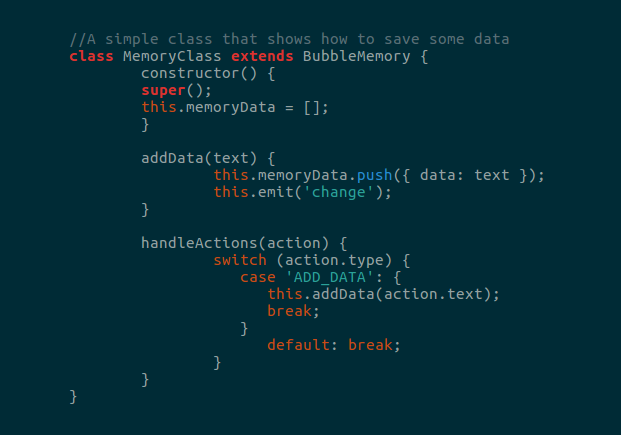
\includegraphics[width=14cm]{../../documenti/UserManualFramework/framework_model/4framework_model_memory.png}
	\caption{BubbleMemory}
\end{figure}

\subsubsection{MatchRegularExpr}
MatchRegularExpr store a regular expression and let the user execute different methods of MatchRegularExpr on some text using it.
It can either operate in Case Sensitive Mode, Multy Line mode and execute multiple matches for a given text.
MatchRegularExpr can combine strings and regexp to create other MatchRegularExpr objects.
\begin{figure}[H]
	\centering
	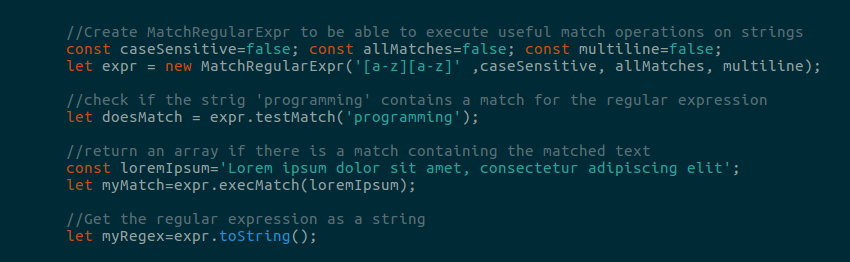
\includegraphics[width=14cm]{../../documenti/UserManualFramework/framework_model/5framework_model_regexp1.png}
	\caption{MatchRegularExpr}
\end{figure}

\begin{figure}[H]
	\centering
	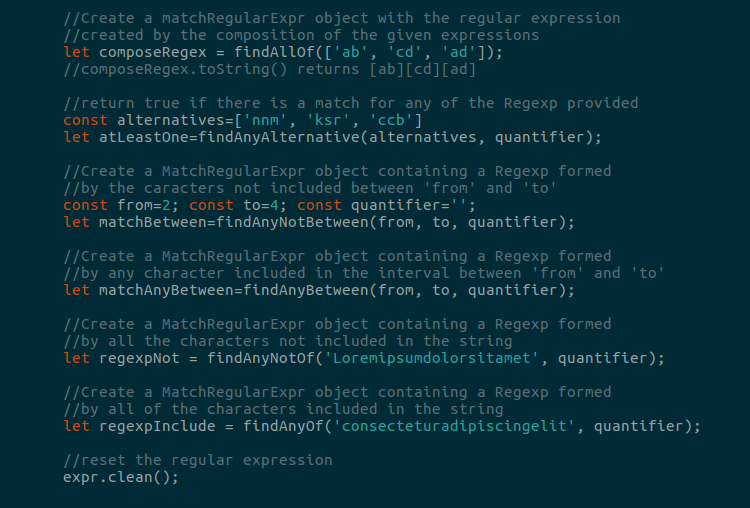
\includegraphics[width=14cm]{../../documenti/UserManualFramework/framework_model/6framework_model_regexp2.png}
	\caption{Regular Expressions}
\end{figure}

\subsection{Graphical Elements}
\subsubsection{Button}
In a Button tag it is possible to specify a text for the button and a to bind a function itha will be called when the button is clicked.
\begin{figure}[H]
	\centering
	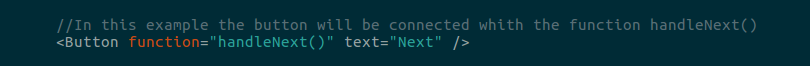
\includegraphics[width=14cm]{../../documenti/UserManualFramework/framework_view/11framework_view_button.png}
	\caption{Button}
\end{figure}

\subsubsection{Label}
A Label can be associated to an HTML element, it can cointain some infomrative text regarding the element.
\begin{figure}[H]
	\centering
	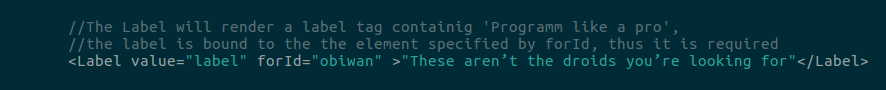
\includegraphics[width=14cm]{../../documenti/UserManualFramework/framework_view/12framework_view_label.png}
	\caption{Label}
\end{figure}

\subsubsection{Image}
Image render an image file and contains a caption describing that image.
\begin{figure}[H]
	\centering
	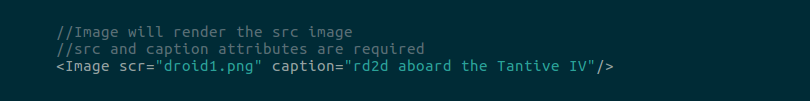
\includegraphics[width=14cm]{../../documenti/UserManualFramework/framework_view/13framework_view_image.png}
	\caption{Image}
\end{figure}

\subsubsection{TextView}
A TextView is a container for some text.
\begin{figure}[H]
	\centering
	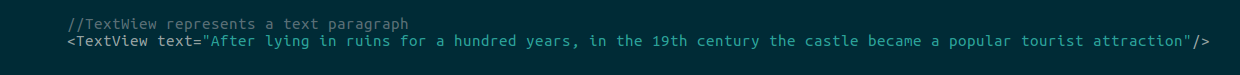
\includegraphics[width=14cm]{../../documenti/UserManualFramework/framework_view/14framework_view_textview.png}
	\caption{TextView}
\end{figure}

\subsubsection{TextEdit}
A TextEdit contains a text paragraph and permits the user to interect whith it, it is possble to bind a function to handle the editing.
\begin{figure}[H]
	\centering
	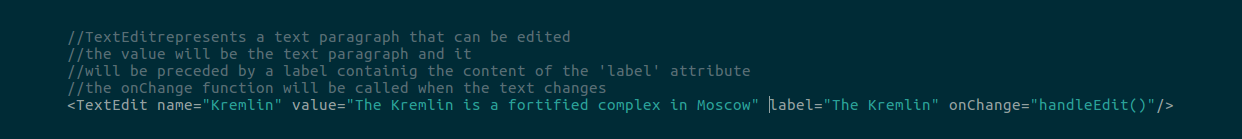
\includegraphics[width=14cm]{../../documenti/UserManualFramework/framework_view/15framework_view_textedit.png}
	\caption{TextEdit}
\end{figure}

\subsubsection{InputText}
InputText renders an input field for strings.
\begin{figure}[H]
	\centering
	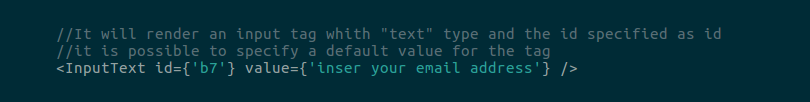
\includegraphics[width=14cm]{../../documenti/UserManualFramework/framework_view/16framework_view_inputtext.png}
	\caption{InputText}
\end{figure}

\subsubsection{InputFile}
InputText renders an input field for a file.
\begin{figure}[H]
	\centering
	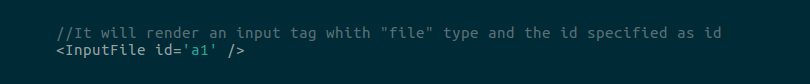
\includegraphics[width=14cm]{../../documenti/UserManualFramework/framework_view/17framework_view_inputfile.png}
	\caption{InputFile}
\end{figure}

\subsubsection{RadioButton}
RadioButton represents a single istance of a button that will be placed togheter whith others RadioButtons either in RadioButtonGroup or in a simple sequence of radioButtons.
\begin{figure}[H]
	\centering
	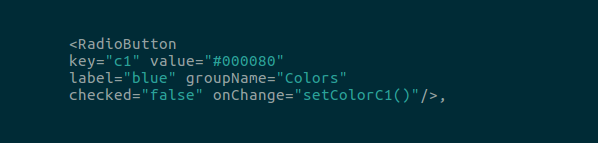
\includegraphics[width=14cm]{../../documenti/UserManualFramework/framework_view/7framework_view_radio.png}
	\caption{RadioButton}
\end{figure}

\subsubsection{RadioButtonGroup}
RadioButtonGroup represents a collection of RadioButtons.
RadioButtonGroup will require di user of the GUI to select a single RadioButton among RadioButtons.
\begin{figure}[H]
	\centering
	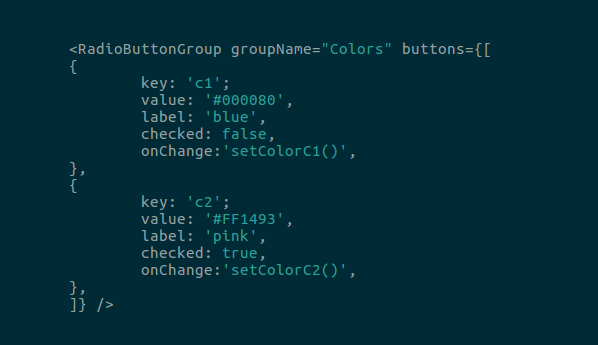
\includegraphics[width=14cm]{../../documenti/UserManualFramework/framework_view/8framework_view_radio_group.png}
	\caption{RadioButtonGroup}
\end{figure}

\subsubsection{CheckBox}
CheckBox represents a single istance of a button that will be placed togheter whith others checkBoxes either in a CheckBoxGroup or in a simple sequence of CheckBoxes.
\begin{figure}[H]
	\centering
	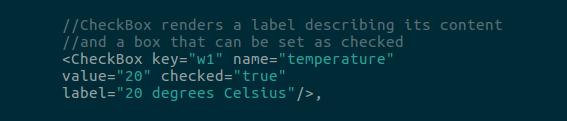
\includegraphics[width=14cm]{../../documenti/UserManualFramework/framework_view/9framework_view_check.png}
	\caption{checkBox}
\end{figure}

\subsubsection{CheckBoxGroup}
CheckBoxGroup represents a collection of CheckBoxes.
CheckBoxGroup will allow the user the user of the GUI to select any number of CheckBoxes.
\begin{figure}[H]
	\centering
	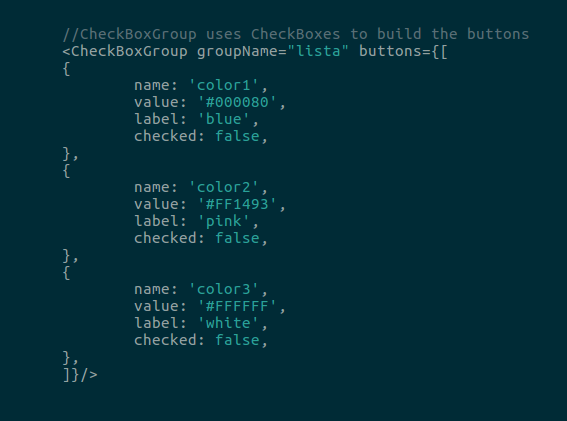
\includegraphics[width=14cm]{../../documenti/UserManualFramework/framework_view/10framework_view_check_group.png}
	\caption{CheckBoxGroup}
\end{figure}

\subsubsection{BarChart}
BarChart presents data whith bars proportional to the values that they represent. It is possible to select colors and grid limits.
\begin{figure}[H]
	\centering
	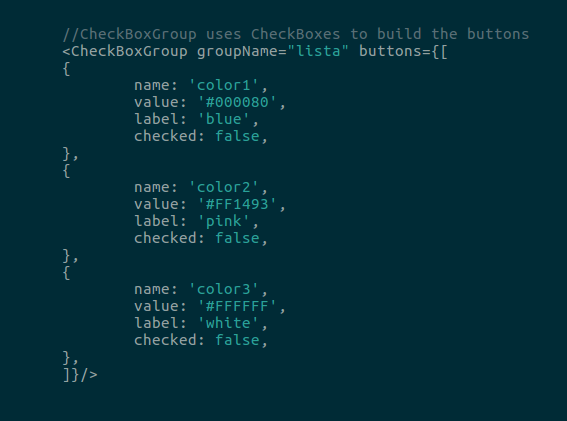
\includegraphics[width=14cm]{../../documenti/UserManualFramework/framework_view/10framework_view_check_group.png}
	\caption{BarChart}
\end{figure}

\subsubsection{PieChart}
PieChart is a circular graphic which is divided into slices. It is possible to specify dimensions and colors for the pie chart. 
\begin{figure}[H]
	\centering
	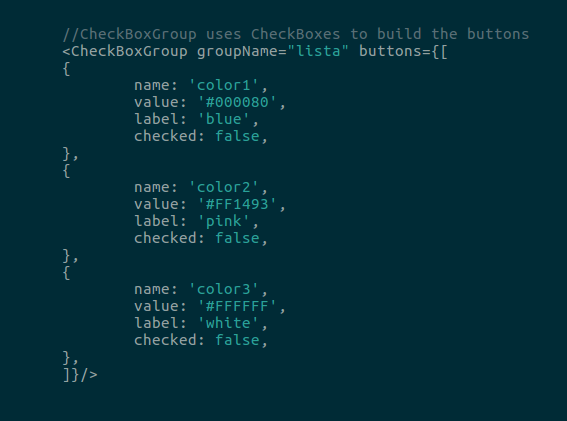
\includegraphics[width=14cm]{../../documenti/UserManualFramework/framework_view/10framework_view_check_group.png}
	\caption{PieChart}
\end{figure}
